\chapter{Technical solution}
\label{cha:techsol}
\lettrine[lines=4, loversize=-0.1, lraise=0.1]{T}{his chapter} will discuss the technical solution and implementation choices made. The chapter will give an overview of the system architecture, and continue on to present the individual parts. The chapter will also cover some solutions in detail and present example data from the system.

\section{System Architecture}
The overall architecture exists of clients and a server (called SpeechServer). The client is an application implemented in Java for the Android platform. The client is the GUI that interacts between the user-input and the SpeechServer. Between the client and the SpeechServer a connection is established by TCP/IP and sends strings captured through the speech recognizer on the smart device. The strings that are sent between SpeechServer and the client follows an internal protocol which is described in Section~\ref{sec:comprot}.

\begin{figure}[h]
\centering
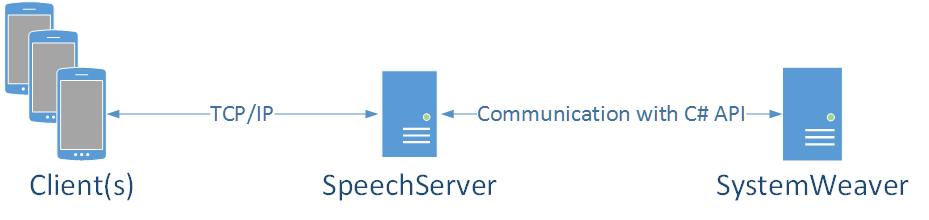
\includegraphics[width = 400pt, keepaspectratio = true]{fig/SystemOverview}
\caption{Architectural overview.}
\label{fig:archoverview}
\end{figure}
\FloatBarrier
SpeechServer is the connection between the client and the requirements in SystemWeaver. SpeechServer interacts with SystemWeaver through a C\#-API provided by Systemite. This allows for SpeechServer to take input from the client and work with the requirement entities in SystemWeaver.

\section{Client}
All user interaction is performed with the client application in SpeechWeaver system, which is developed for Android 4.1 and above to facilitate offline voice typing \citep{offlvoice}.  However, because of the string based communication, the system does not require an Android based client, only that the client can send and receive TCP/IP messages.
Hence, it is possible to develop clients for different platforms, e.g. desktop applications or web applications, in order to take advantage of their respective advantages in different use cases.
However, in this project the focus has been on smartphones in order to take advantage of the mobility that they provide.
Therefore all further references in this article to ``the client''  will refer to the developed Android client.

\subsection{Usage}
\label{subsec:usage}
The client follows the protocol as described in Section~\ref{sec:comprot}. Within the application, information that is sent from the server to the client is spoken by the application by Android's text-to-speech engine. Before the user can interact with the requirement database, the user types in and sends user credentials (username and password) to the SpeechServer for validation in SystemWeaver. Once the client is authorized, the user is presented with available projects and the user taps to select the project that user wants to search in. Once a project has been selected, there are three possible actions that can be taken, either: 
\begin{enumerate}
\item Annotating a requirement - By tapping a button and provide the server with a requirement ID and then an annotation (through their speech)
\item Annotating a requirement with extra data - By selecting a file from the smart device (e.g.\ a picture or a recorded sound file) and after that proceeding with the actions mentioned in 1. After those actions are done the application also uploads the selected file to the SpeechServer.
\item Generate a report - By tapping a button which triggers the SpeechServer to generate a report (see section ~\ref{sec:repgen}).
\end{enumerate}
\\
A picture illustrating the client's flow can be seen below in Figure \ref{fig:clientflow}

\begin{figure}[h]
\centering
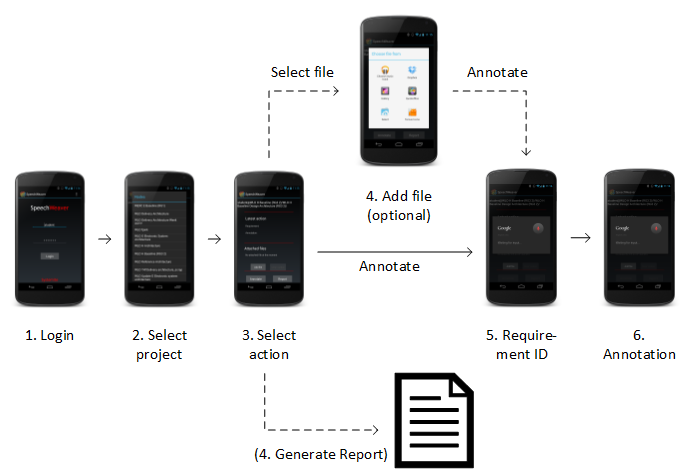
\includegraphics[width = 400pt, keepaspectratio = true]{fig/ClientFLOWupdated}
\caption{The sequence flow of the client}
\label{fig:clientflow}
\end{figure}
\FloatBarrier

The use of auditory interaction with SpeechWeaver removes all need for the user to focus on the application. When the server expects input from a client, an identifier and an explanatory string is sent to the user which is then spoken by the application through Android's text-to-speech-engine. However, to start any of the above mentioned actions, the user needs to tap a button on the screen. Action 1, \emph{Annotate a requirement} can however also be initiated through the button on a bluetooth headset.
Thus facilitating concurrent usage of the system during, for instance, requirements review.
\subsection{Speeech Recognition}
\label{sec:sr}
The Android application captures the users voice using the built in API for speech recognition \citep{recAPI}.
When launching the speech recognizer, a pop up dialog appears and a sound is generated to inform the user that the speech recognizer is ready to capture input.
%The user can then state/input a desired phrase. 
The speech recognizer will then record the users input until it does not receive any new input for one second, i.e.\ until the user goes silent after stating the desired phrase. 
This event will cause the pop up dialog to close and a sound is generated to to inform the user that the speech recognizer has caught the input and is processing it. 
When the speech recognizer has processed the input, it returns up to five results. 
These results are based on how confident the recognizer is that the returned result was correct, where the first of the five results is what the recognizer interpreted as the most likely input from the user. An example of the results from a speech recognizer can be seen below in Table~\ref{tab:fiveresults}

\begin{table}[h]
\centering
\caption{The five results returned from Android's speech recognizer for the input "Speech recognizer and confidence scores.}
    \begin{tabular}{ l  l }
        \hline
        Rank & Result \\
        \hline
        1 & Speech recogniser and confidence scores \\
        2 & Speech recognizer and confidence scores\\
        3 & Speech recogniser and confidential scores\\
        4 & Speech recogniser and confidence course\\
        5 & Speech recognizer and confidential scores\\
        \end{tabular}
\label{tab:fiveresults}
\end{table}

All five alternative user input strings are then sent to the SpeecServer for post-processing.

Android's standard speech recognizer supports different languages. 
However, through out this project, English US was selected used as the primary input language, meaning that the domain of possible interpretations for the speech recognizer were words from the american english dictionary. 
In addition to this dictionary, the speech recognizer also provides the commands "period", "comma", "exclamation mark/point" and "question mark" which are translated into their corresponding characters \citep{typetextbyspeaking}.

\section{Communication Protocol}
\label{sec:comprot}
The communication between SpeechServer and the clients is handled by a custom protocol built on tags that represent different states in the communication. 
The tags are sent over a TCP/IP-socket and are interpreted at the receiving end.
The tags attached to the messages are dependent on which state the system currently is in, i.e. when the client trigger the annotation by sending a requirement title, the messages is tagged with ID (Identification). When the server has found a requirement title (the ID), it returns a message with the tag WFT (Waiting For Tag) and the next output containing the annotation from the client to the server is tagged with ANOT (Annotation). 
%EA: what does dependent on which state the system currently is in mean? Does it mean that the tags change based on the state of client/server? Or does it mean that the tags can only be recieved when the client/server is in a specific state? Clarify and elaborate this a little to give the reader a better understanding of how the tags work and what they represent.

During the setup-phase, after a connection has been established between the client and the server and the user has logged into the system, the server acts as the active part to form a context for the whole system to work within. 
Once the setup-phase is over, SpeechServer takes a passive role where different operations are triggered based on the what is received from the client. % it starts different communication states dependent on what the client send. 
%However, the passive role of the server enabled the communication states to be decided from the client and do not need to be strictly followed if the client decides to abort the current communication-state.
This implementation allows the communication states to be decided from the client and also means that they don't need to be followed if the client decides to abort the current communication state. Once the setup-phase is over, operations (sending an ID, sending an annotation, create a report etc) are always triggered by the client. The different operations can at any point be aborted and re-selected by the client.
\section{SpeechServer}
\label{sec:speechserver}
The server is written in C\# and has one thread for each client and can handle multiple clients simultaneously. Since SystemWeaver is a real time collaboration tool used in the industry that handles large requirements databases, the API and SystemWeaver can handle many simultaneous users with ease. Clients connect to SpeechServer by sending input to a predefined socket that the server listens to.
User authentication, in turn, is handled by checking with SystemWeaver that the provided username and password are both valid.

\begin{figure}[h]
\centering
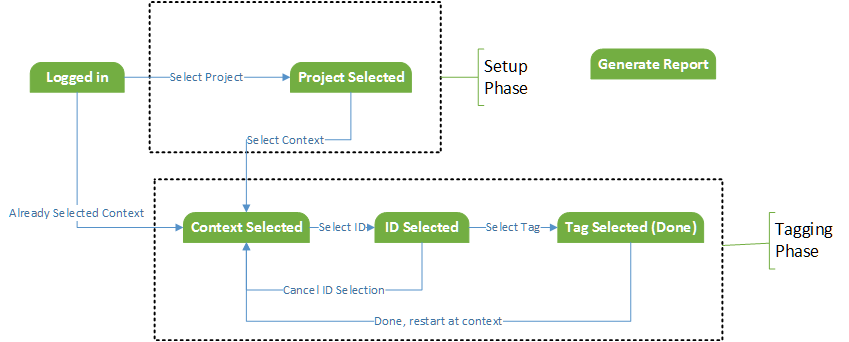
\includegraphics[width = 400pt, keepaspectratio = true]{fig/serverFlow}
\caption{A simplified state machine showing the states of the SpeechServer handling one client.}
\label{fig:serverFlow}
\end{figure}

As soon as a client connects to the server, the client is given a broker-object by the C\# API to be able to interact with SystemWeaver. 
The broker provides the client with all necessary operations to interact with SystemWeaver, such as authentication, fetching items/parts and writing to SystemWeaver through a connection that is kept alive as long as the client stays connected. 

The flow in the server is described by a simplified state machine shown in Figure~\ref{fig:serverFlow}. If the client has not provided a project to work in, the server fetches all the projects with the broker, and sends all available projects to the client and asks which project to work in. The contexts from a selected project, which is a delimited part of a project or an abstraction level (e.g.\ Analysis Level, Design Level, Implementation Level) are treated in the same way by the user, but is traversed to from the project node. The server sends all context within that project and the user selects one. This is the \emph{Setup Phase} which is accessible from all other states if the user should choose to change.

After the setup phase, the \emph{Annotation Phase} begins, this is where the system adds the annotations. As the client provides an ID-tag together with the string input for the title of the requirement, the SpeechServer tries to locate it using methods described further in Section~\ref{sec:nlp}. When the name is found on the server it stores this temporarily, and asks the client for what annotation to annotate the requirement with. When the annotation is chosen by the user it gets processed into the one of the predefined annotations in the server and annotates the requirement with the specified annotation by adding an issue to the requirement via the C\#-API of SystemWeaver.

\subsection{Finding a Requirement Using Natural Language Processing}
\label{sec:nlp}
When the server processes the string input it does it in several steps and is dynamic depending on its accuracy of the results. Using name input as the example in the following scenario we will describe the process. The client provides several strings for interpreted results in the order of likelihood (weighted on the confidence scores as described in~\ref{sec:sr}). First the server looks for a perfect string match for the five inputs. If no perfect matches were found, the Levenshtein distance algorithm as described in~\ref{subsubsec:stringmetric} is used to find the most similar string, from now on called closest matches, on the most likely interpreted result from the speech recognizer. Then the server returns the closest matches sorted by their Levenshtein distance from the input string so the user can choose from these.

There are a few reasons why not to handle the entire input string in one message (as described in the Section~\ref{sec:natlangprocsess}). The first reason is that there are problems breaking the input string down in its parts since it's complicated to find which part of the string is the id, and what parts are annotations. If the system would have listened for special syntax (example highlighted in bold) such as:

\begin{framed}
\begin{flushleft}
\emph{\textbf{Requirement:} "System should not create a file." \textbf{Annotation: "Ambiguous"}}
\end{flushleft}
\end{framed}

there is a possibility that the requirement could contain these keywords or other syntax words which would result in a faulty delimitation of the string. 
The second reason is that a single string solution requires more from  the user since he/she needs to remember and formulate the syntax, keywords, requirement ID and the annotation before speaking~\citep{memoryCap}. 
Having separated the input into different stages lessens the burden for the system to compensate for these issues, as well as lessen the burden for the user since the user now only needs to answer the questions stated by the application. 
The question-response communication implementation also makes failure mitigation easier if an operation fails since the user can quicker just abort or retry the operation.

\subsubsection{String Edit Distance Function - Levenshtein distance}
\label{subsubsec:stringmetric}
A way of improving the speech recognizer is to add an algorithm which gives us an indication of what input the user \emph{wanted}, as opposed to what the speech recognizer interpreted. When searching for entities within a finite interval, as in the example with requirement names in a requirement database, we improve this by measuring a string edit distance (see Section~\ref{subsec:sedf}) between the interpreted input from the speech recognizer and the values in the target domain. This allows us to narrow down the number of possible results and thereby identify the correct result with higher certainty.

In Levenshteins string distance function, whether you add, delete or modify a character within a string, it is calculated as a cost of one. An string edit distance derived from an algorithm where this property is fulfilled is often called a Levenshtein distance \citep{blockeel2004}. 

\begin{figure}
\centering
    The distance between two strings \(x,y\) given by \(\operatorname{lev}_{x,y}(|x|,|y|)\) where \\  
    $\qquad\operatorname{lev}_{x,y}(i,j) = \begin{cases}
      \max(i,j) &, \min(i,j)=0 \\
      \min \begin{cases}
              \operatorname{lev}_{x,y}(i-1,j) + 1 \\
              \operatorname{lev}_{x,y}(i,j-1) + 1 \\
              \operatorname{lev}_{x,y}(i-1,j-1) + [x_i \neq y_j]
           \end{cases} &, \text{ else}
    \end{cases}
    $
    \caption{The edit-distance (Levenshtein distance) between two strings, \emph{x},\emph{y}, where all operations has a cost of one.}
\end{figure}

In our system we use Levenshtein distances when a given input \emph{x} does not have a a requirement name that perfectly matches \emph{x}. We then calculate the distance between \emph{x} and all requirements in the given database and returns a set of requirements with the lowest Levenshtein distances, and the user can then chose which requirement the user originally sought.

\section{Annotations}
In order to create high quality software requirements specifications (SRS), IEEE have developed a recommended practice for SRSs~\citep{IEEE830}. The guideline also shows how the practice connects to software lifecycle processes~\citep{IEEE12207}. The decision was to use chapter \textit{4.3 - Characteristics of a good SRS} from IEEE Recommended Practice for Software Requirements Specifications as the basis for the annotations. 

The definition of a high quality SRS used in the context of SpeechWeaver is that all requirements and requirement groups should conform to the characteristics described in Table~\ref{tab:anots}. This is somewhat broader than the practice since it only discusses the whole SRS and the particular requirements, not intermediate collections of requirements and individual requirements. 

\begin{table}[h]
\centering
\caption{IEEE Quality Characteristics and the corresponding SpeechWeaver Annotations.}

    \begin{tabular}{ l  l }
        \hline
        IEEE Quality Characteristics & SpeechWeaver Annotations \\
        \hline
        Unambiguous & Ambiguous \\
        Correct & Incorrect \\ 
        Complete & Incomplete \\
        Consistent & Inconsistent \\
        Ranked for importance and/or stability & Unprioritized \\
        Verifiable & Unverifiable \\
        Modifiable & Unmodifiable \\
        Traceable & Untraceable \\
        \end{tabular}   
\label{tab:anots}
\end{table}

The annotations provided are the complementary antonyms of these characteristics, with the exception of \emph{Unprioritized} since it captures the meaning better, is a single word and is more understandable in natural language. These annotations are just a suggestion that captures many of the problems a requirement can have. This is customizable per customer and organization, to suit problems that a particular organization encounters. This is also customizable in run time and can be changed and perfected continuously during a project to give more narrow definitions of the annotations. It is also possible to have synonyms to the annotation tags, so that a user can say \emph{"Not clear."} or \emph{"Not well defined"} instead of \emph{"Ambiguous"}. This reduces the burden to remember exact syntax, but all these synonyms maps to the same tag within the system, that is \emph{Ambiguous}. This is needed to be able to interpret the tags in the same way, as well as to be able to sort and filter within SystemWeaver and extract the annotations for aggregations in the report generation.

\FloatBarrier
\section{Report Generation}
\label{sec:repgen}
The annotations made by the users are stored in SystemWeaver as individual entities, this allows several users to annotate the same requirement with the same annotation several times. These annotations are stored in an \emph{issue} (see section \ref{subsec:issue})connected to the requirement, and the connection can be traversed in any direction. The report generation uses these annotations while iterating over the report structure. The output of the report generation are the statistics for the requirements and how many have been annotated with the different annotations. An example can be seen in Table~\ref{tab:repgenstat1} and Table~\ref{tab:repgenstat2}. Note that the first table shows how many requirements are tagged with the different annotations. This means that if a requirement is annotated several times with the same tag by different users, i.e.\ several people think that a requirement is \textit{ambiguous}, then the annotation is only counted once for that requirement, to see the status over all requirements. This also means that one requirement can be represented in all categories. In the other table we see the total number of annotations, i.e all annotations are counted.

\begin{table}[h]
\centering
\caption{Example statistics from report generation output, annotated requirements.}
    \begin{tabular}{ l l l}
        \hline
        SpeechWeaver Annotations & Tagged RQs & \% \\
        \hline
        Ambiguous & 5 & 1\% \\ 
        Incorrect & 10 & 2\%  \\ 
        Incomplete & 50 & 10\%  \\ 
        Inconsistent & 1 & 0.2\%  \\
        Unprioritized & 10 & 2\%  \\
        Unverifiable & 100 & 20\%  \\
        Unmodifiable & 20 & 4\%  \\
        Untraceable & 80 & 16\%  \\ \hline
        \textbf{Total: Annotated requirements} & \textbf{276} & \\
        \textbf{Total: Requirements} & \textbf{500} & \\
        \end{tabular}     
\label{tab:repgenstat1}
\end{table}

\begin{table}[h]
\centering
\caption{Example statistics from report generation output, statistics on annotations.}
    \begin{tabular}{ l l l}
        \hline
        SpeechWeaver Annotations & Annotation Count & \% \\
        \hline
        Ambiguous & 10 & 3.3\% \\ 
        Incorrect & 20 & 6.7\%  \\ 
        Incomplete & 60 & 20\%  \\ 
        Inconsistent & 5 & 1.6\%  \\
        Unprioritized & 15 & 5\%  \\
        Unverifiable & 110 & 36.7\%  \\
        Unmodifiable & 30 & 10\%  \\
        Untraceable & 50 & 16.7\%  \\ \hline
        \textbf{Total: Annotations} & \textbf{300} & \\
        \end{tabular} 
\label{tab:repgenstat2}
\end{table}

The generated report also gives annotations grouped in a headline so the reader can see all requirements annotated with a specific annotation. Furthermore there is headlines for each requirement so the reader can see what problems a particular requirement has. The output shows the description for each requirement so the review process is simple. 

The annotations can also be shown for specific time periods or iterations, depending on the project setup. This means that statistics can be shown over time and the data can be plotted to see the history and development of the annotations.
















